\documentclass[tikz]{standalone}
\usepackage{tikz} 
\usetikzlibrary{shapes.misc,patterns,hobby}
\usepackage{pgfplots}
\usepgfplotslibrary{fillbetween}
%\usepackage[active,tightpage]{preview}  %generates a tightly fitting border around the work
%\PreviewEnvironment{tikzpicture}
%\setlength\PreviewBorder{2mm}
\usepackage{xcolor}
\definecolor{myred}{RGB}{196,19,47} 
\definecolor{myblue}{RGB}{0,139,139}

\begin{document}
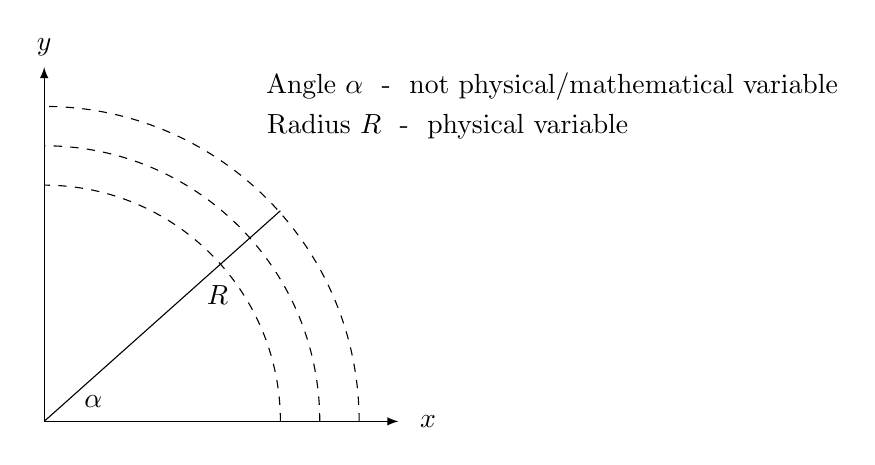
\begin{tikzpicture}[xscale=2.5,yscale=2.5,>=latex]

%Koordinatensystem 
\draw[->, thin] (0,0) to (1.8,0);
\node at (1.95,0) {$x$};
\draw[->, thin] (0,0) to (0,1.8);
\node at (0,1.9) {$y$};
  
%Kreise
\newcommand\kreis{\node[draw=black,dashed,circle,inner sep=0pt, minimum size = 6cm] (0,0) {}}
\newcommand\kreiss{\node[draw=black,dashed,circle,inner sep=0pt, minimum size = 7cm] (0,0) {}}
\newcommand\kreisss{\node[draw=black,dashed,circle,inner sep=0pt, minimum size = 8cm] (0,0) {}}
\begin{scope}[]
\clip[] (0,0) rectangle (2,2);
\kreis;
\kreiss;
\kreisss;
\end{scope}

%Winkel
\draw[-, thin] (0,0) to (1.2,1.07);
\node at (0.25,0.1) {$\alpha$};
\node at (0.88,0.64) {$R$};

\node at (2.58,1.7) {Angle $\alpha$ \ - \ not physical/mathematical variable};
\node at (2.05,1.5) {Radius $R$ \ - \ physical variable};



\end{tikzpicture}
\end{document}